% bei Standalone in documentclass noch:
% \RequirePackage{luatex85}

\documentclass[captions=tableheading, titlepage= firstiscover, parskip = half , bibliography=totoc]{scrartcl}
%paper = a5 für andere optinen
% titlepage= firstiscover
% bibliography=totoc für bibdateien
% parskip=half  Veränderung um Absätze zu verbessern

\usepackage{scrhack} % nach \documentclass
\usepackage[aux]{rerunfilecheck}
\usepackage{polyglossia}
\usepackage[style=numeric, backend=biber]{biblatex} % mit [style = alphabetic oder numeric] nach polyglossia
\addbibresource{lit.bib}
\setmainlanguage{german}

\usepackage[autostyle]{csquotes}
\usepackage{amsmath} % unverzichtbare Mathe-Befehle
\usepackage{amssymb} % viele Mathe-Symbole
\usepackage{mathtools} % Erweiterungen für amsmath
\usepackage{fontspec} % nach amssymb
% muss ins document: \usefonttheme{professionalfonts} % für Beamer Präsentationen
\usepackage{longtable}

\usepackage[
math-style=ISO,    % \
bold-style=ISO,    % |
sans-style=italic, % | ISO-Standard folgen
nabla=upright,     % |
partial=upright,   % /
]{unicode-math} % "Does exactly what it says on the tin."
\setmathfont{Latin Modern Math}
% \setmathfont{Tex Gyre Pagella Math} % alternativ

\usepackage[
% die folgenden 3 nur einschalten bei documenten
locale=DE,
separate-uncertainty=true, % Immer Fehler mit ±
per-mode=symbol-or-fraction, % m/s im Text, sonst \frac
]{siunitx}

% alternativ:
% per-mode=reciprocal, % m s^{-1}
% output-decimal-marker=., % . statt , für Dezimalzahlen

\usepackage[
version=4,
math-greek=default,
text-greek=default,
]{mhchem}

\usepackage[section, below]{placeins}
\usepackage{caption} % Captions schöner machen
\usepackage{graphicx}
\usepackage{grffile}
\usepackage{subcaption}

% \usepackage{showframe} Wenn man die Ramen sehen will

\usepackage{float}
\floatplacement{figure}{htbp}
\floatplacement{table}{htbp}

\usepackage{mhchem} %chemische Symbole Beispiel: \ce{^{227}_{90}Th+}


\usepackage{booktabs}

 \usepackage{microtype}
 \usepackage{xfrac}

 \usepackage{expl3}
 \usepackage{xparse}

 % \ExplSyntaxOn
 % \NewDocumentComman \I {}  %Befehl\I definieren, keine Argumente
 % {
 %    \symup{i}              %Ergebnis von \I
 % }
 % \ExplSyntaxOff

 \usepackage{pdflscape}
 \usepackage{mleftright}

 % Mit dem mathtools-Befehl \DeclarePairedDelimiter können Befehle erzeugen werden,
 % die Symbole um Ausdrücke setzen.
 % \DeclarePairedDelimiter{\abs}{\lvert}{\rvert}
 % \DeclarePairedDelimiter{\norm}{\lVert}{\rVert}
 % in Mathe:
 %\abs{x} \abs*{\frac{1}{x}}
 %\norm{\symbf{y}}

 % Für Physik IV und Quantenmechanik
 \DeclarePairedDelimiter{\bra}{\langle}{\rvert}
 \DeclarePairedDelimiter{\ket}{\lvert}{\rangle}
 % <name> <#arguments> <left> <right> <body>
 \DeclarePairedDelimiterX{\braket}[2]{\langle}{\rangle}{
 #1 \delimsize| #2
 }

\setlength{\delimitershortfall}{-1sp}

 \usepackage{tikz}
 \usepackage{tikz-feynman}

 \usepackage{csvsimple}
 % Tabellen mit \csvautobooktabular{"file"}
 % muss in table umgebung gesetzt werden


% \multicolumn{#Spalten}{Ausrichtung}{Inhalt}

\usepackage{hyperref}
\usepackage{bookmark}
\usepackage[shortcuts]{extdash} %nach hyperref, bookmark

\newcommand{\ua}[1]{_\symup{#1}}
\newcommand{\su}[1]{\symup{#1}}


\begin{document}

\section{Auswertung}

Im Folgendem werden die Messergebnisse ausgewertet und in geeigneter
Weise visualisert.

\subsection{Grezfrequenzen}

Die verwendete Apparatur hatte die folgenden Werte.

\begin{align}
  \label{L}
  L &= \SI{1,217}{\milli\henry}\\
  \label{C1}
  C_1 &= \SI{20,13}{\nano\farad}\\
  \label{C2}
  C_2 &= \SI{9,41}{\nano\farad}
\end{align}

Diese Daten wurden ohne Fehler angegeben und werden deshalb als fehlerfrei
angenommen. In der $LC$-Kettenschaltung wurde der Kondensator mit der
Kapazität $C_1$ verwendet.

Mittels der Formeln ????? ergeben dich die die Grenzfrequenzen zu:

\begin{align*}
  \omega_{Grenz,C} &= \num{404075,78}\si{\hertz}\\
  \omega_{Grenz,C_1C_2}^{akustisch} &= \num{285724,72}\si{\hertz}\\
  \omega_{Grenz,C_1C_2}^{optisch} &= \num{417902,43}\si{\hertz}\\
\end{align*}

Mit Hilfe des $XY$-Scheibers wurden die Grenzfrequenzen der $LC$-Kettenschaltung
und der $LC_1C_2$-Kettenschaltung visualisiert. Die Diagramme sind
logarithmisch. Durch ermitteln der Frequenzen an bestimmten Stellen der
Grafik kann eine Exponentielle Regressionsrechnung gemacht werden.
Damit ist einen Zusammenhang zwischen den Messdaten und vom Generator durchlaufenden
Frequenzen bekannt.

Die Ausgleichsrechnung wurde mithilfe des \emph{Python}-Packetes
\emph{curve\_Fit} bewerkstelligt. Die Funktion hatte die Gestalt.

\begin{equation}
  \nu(t) = a\cdot e^{bx}+c
\end{equation}

Es ergeben sich mittels der Messdaten (??) die folgenden Funktionen.

\begin{align}
  \label{eqn:Ausgleichsrechnung_exp_1}
  \nu_{C}(x) &= (13984\pm 1701)\cdot e^{(0,08\pm 0,005)\cdot x} - (5155\pm 2006) \\
  \label{eqn:Ausgleichsrechnung_exp_2}
  \nu_{C_1C_2}(x) &= (64117\pm 5474)\cdot e^{(0,15\pm 0,005)\cdot x}-(20547\pm 7703)
\end{align}

Anhand der Graphen kann die Grenzfrequenz abgelesen werden, indem der
Abstand vermessen wird. Das Messung wurde mit einem Lineal gemacht
und ergibt für die $LC$-Kettenschaltung einen Wert von ca.
$\SI{17,2}{\centi\meter}$. Die Messung der Grenzfrequenzen der
$LC_1C_2$-Kettenschaltung ergab für den akustischen Zweig eine
Grezfrequenz bei $\SI{11}{\centi\meter}$ und für den optischen Zweig eine
Grenzfrequenz bei  $\SI{12,2}{\centi\meter}$.

Für die Grenzfrequenzen ergeben sich damit die Werte:

\begin{align}
  \omega_{Grenz,C} &= \num{50224,00\pm 3864,40}\si{\hertz}\\
  \omega_{Grenz,C_1C_2}^{akustisch} &= \num{311361,75\pm 13506,32}\si{\hertz}\\
  \omega_{Grenz,C_1C_2}^{optisch} &= \num{376566,51\pm 13543,23}\si{\hertz}
\end{align}

\section{Dispersionskurven}

Mit den Angaben \eqref{L}, \eqref{C1} und \eqref{C2} kann die Dispersionskurve
der $LC-Kette$ und der $LC_1C_2$-Kette über die Funktion (??) bestimmt werden.
Die Messdaten wurden in das Diagramm mit eingetragen.

\begin{figure}
  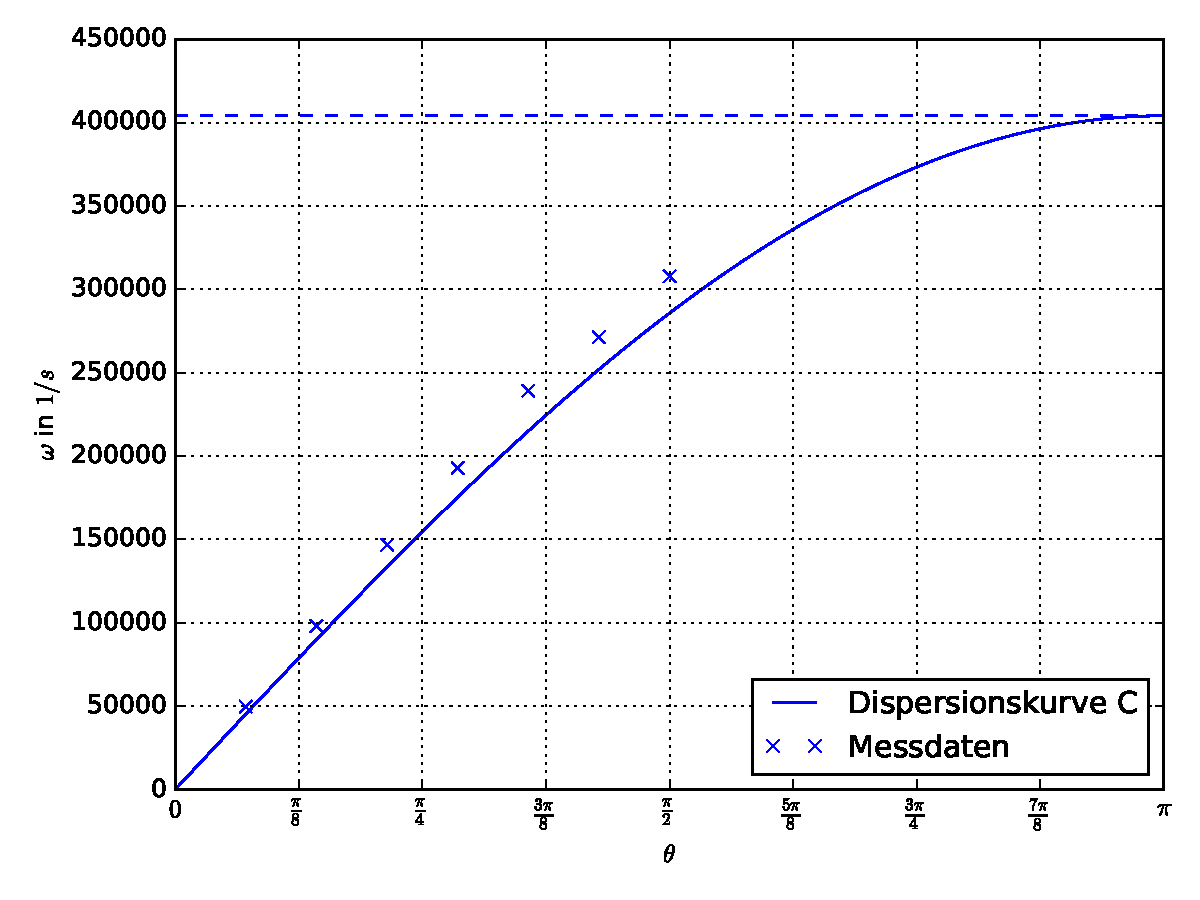
\includegraphics[width=\textwidth]{Dispersionskurve_C.pdf}
  \caption{Dispersionskurve der $LC$-Kettenschaltung}
  \label{fig:DispersionC}
\end{figure}
\begin{figure}
  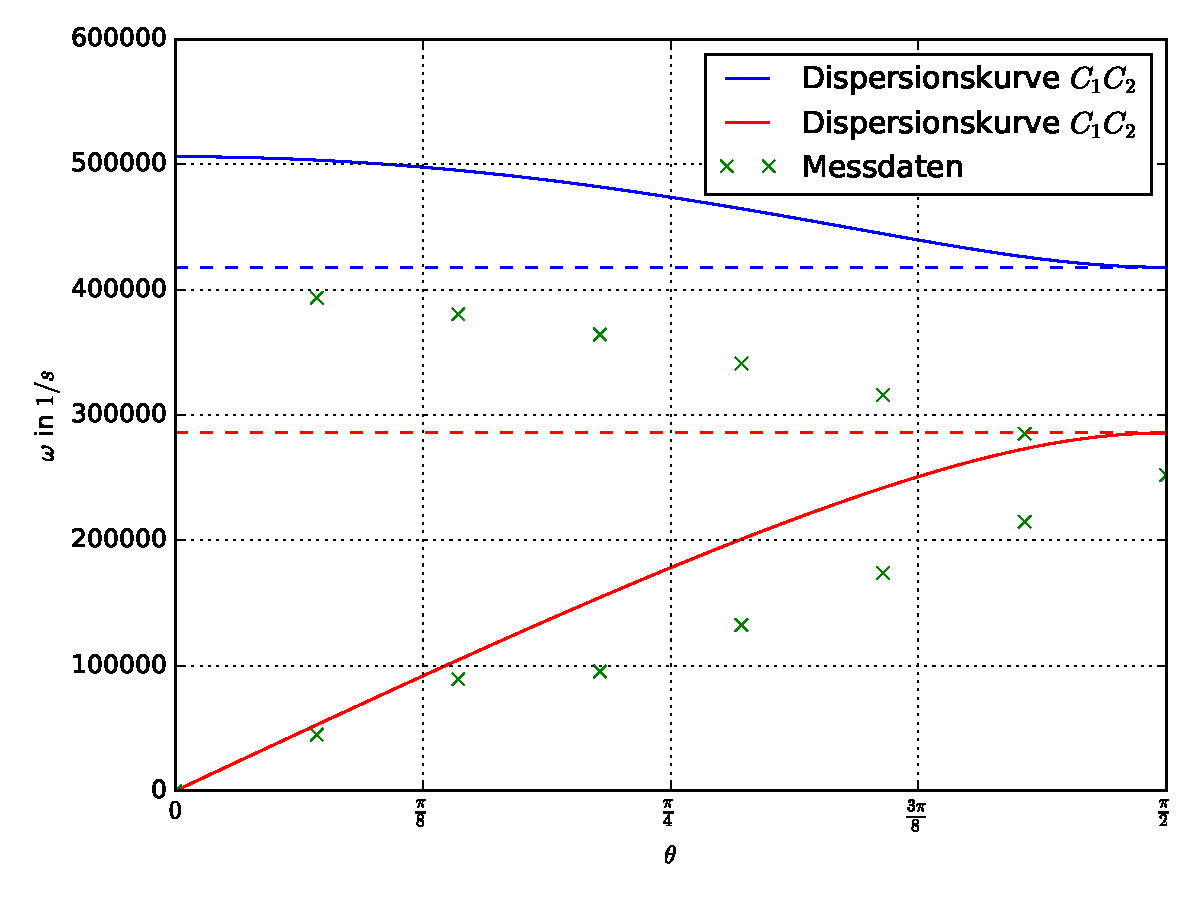
\includegraphics[width=\textwidth]{Dispersionskurve_C1C2.pdf}
  \caption{Dispersionskurve der $LC_1C_2$-Kettenschaltung}
  \label{fig:DispersionC1C2}
\end{figure}
\FloatBarrier

\subsection{Stehende Wellen}

Beim messen der Spannungsamplituden der offenen $LC$-Kette ergeben sich die folgenden
Diagramme.

\begin{figure}
  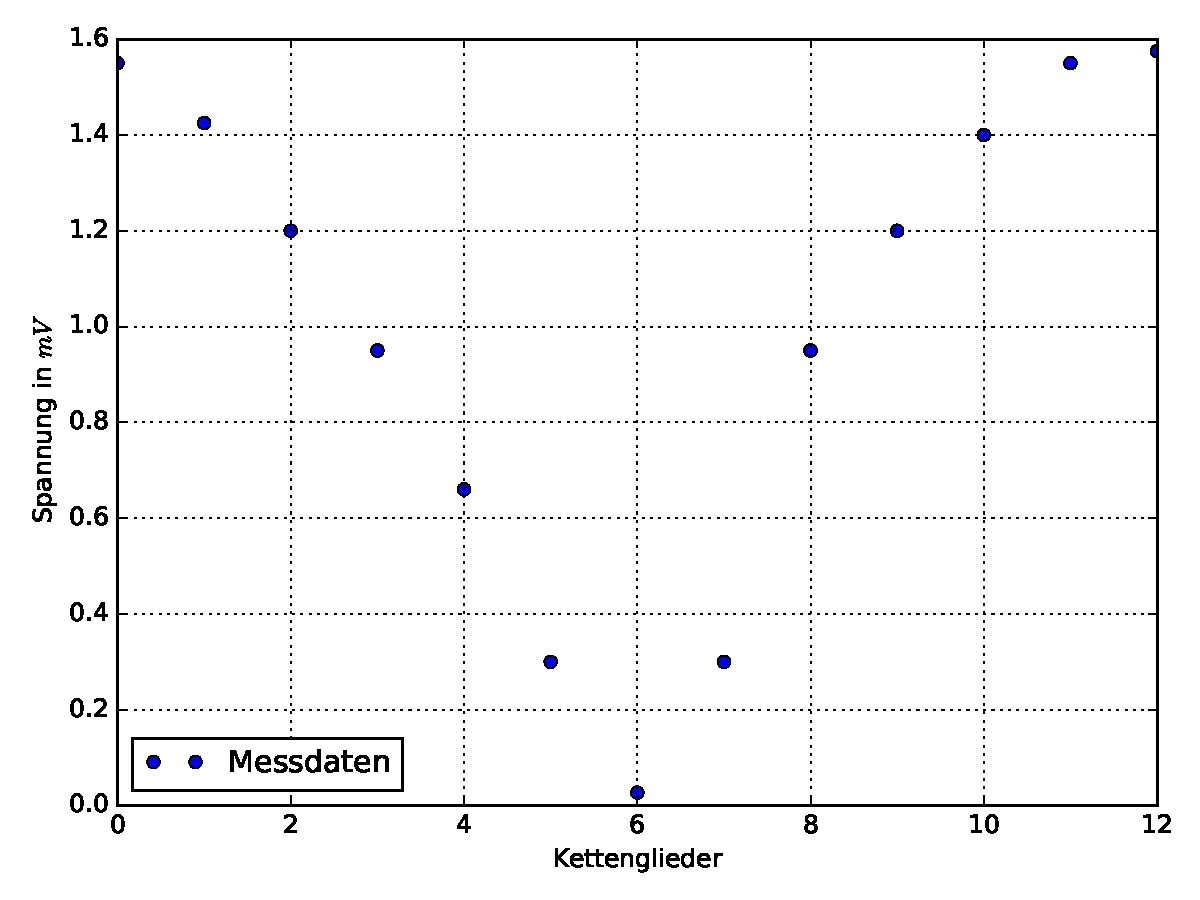
\includegraphics[width=\textwidth]{Messung_d_1.pdf}
  \caption{Erste Grundschwingung der offenen $LC$-Kettenschaltung bei $\nu = \SI{7133}{\hertz}$}
  \label{fig:Messungd1}
\end{figure}

\begin{figure}
  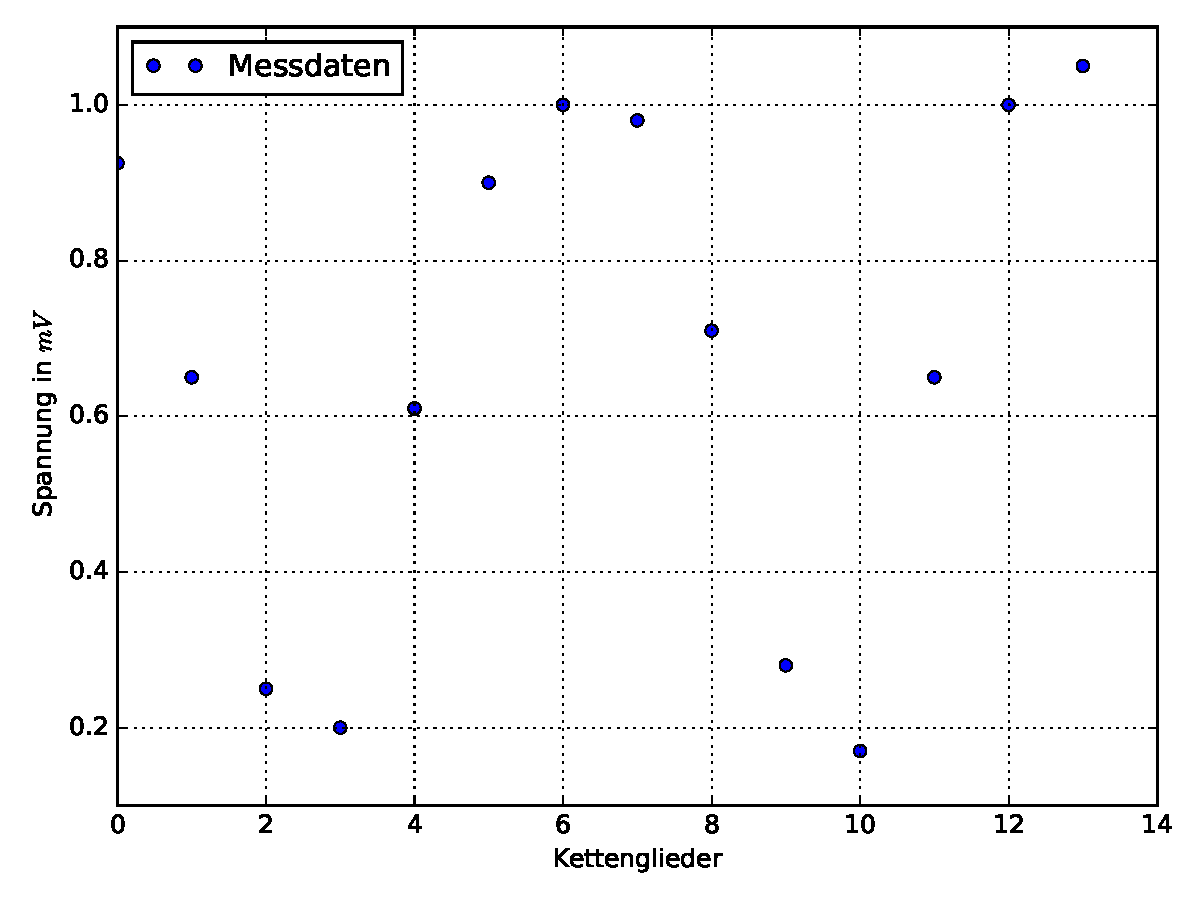
\includegraphics[width=\textwidth]{Messung_d_2.pdf}
  \caption{Zweite Grundschwingung der offenen $LC$-Kettenschaltung bei $\nu = \SI{14307}{\hertz}$}
  \label{fig:Messungd2}
\end{figure}

\begin{figure}
  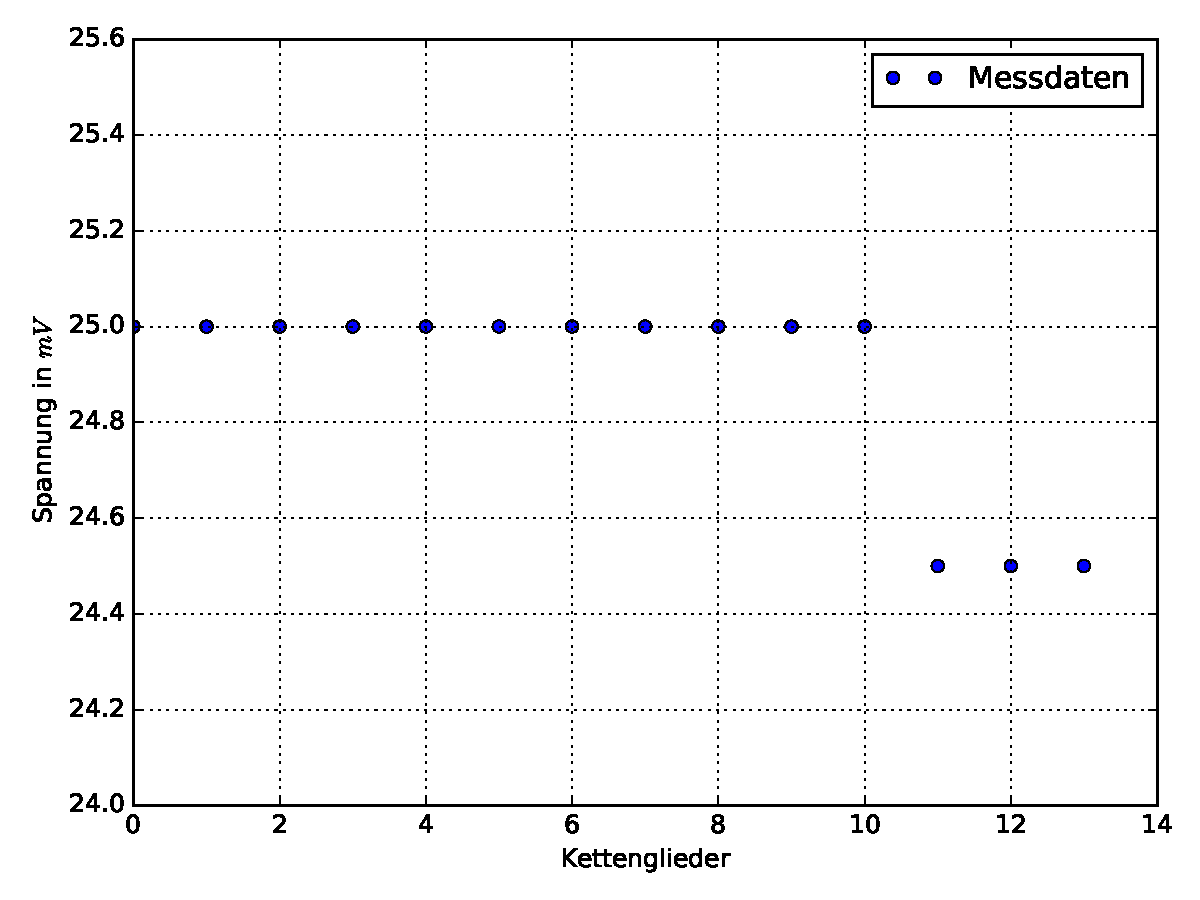
\includegraphics[width=\textwidth]{Messung_e.pdf}
  \caption{Abgeschlossene $LC-$Kettenschaltung bei $\nu = \SI{7337}{\hertz}$}
  \label{fig:Messunge}
\end{figure}

\section{Diskussion}

Im Folgendem werden die Messergebnisse diskutiert.
Zunächst wird auf mögliche Fehlerquellen eingegangen, mit denen sich die Messungenauigkeiten
begründen lassen. Zum einen war das Einstellen des Wellenwiderstandes auf der
Eingangsseite (links) äußert unpräzise. Leichte Berührungen des Widerstandreglers
hatten schon enormen Einfluss auf den widergegebenen Widerstand.
Zudem konnten die gemessenen Frequenzen nur schwierig abgelesen werden, da der
Generator keine kontinuierliche Frequenz bereitgestellt hat. Die Frequenzen
können deshalb die Messergebnisse mit Fehlern behaftet haben.
Während des zeichnens der Durchlasskurve von dem $XY$-Schreibers wurden Fixpunkte
an dem Diagramm gewählt, an denen die Frequenz zu bestimmen war.
Das Messen der Frequenzen erfolgte jedoch nicht parrallel zum Zeichnen.
Insgesamt ist zu sagen, dass die verwendete Apparatur sehr alt ist und sehr
undurchsichtig wirkte.
Die Induktivitäten und Kapazitäten der Apparatur wurden als fehlerfrei angenommen.\\
Die Messergebnisse der Durchlasskurven sind in den Abbildungen \ref{fig:DispersionC}
und \ref{fig:DispersionC1C2} dargestellt. Es ist ersichltich, dass
die Dispersionskurve der $LC$-Kette beinahe auf der Theoriekurve liegt.
Jedoch wird nicht die theoretische Grenzfrequenz in dem Aufbau erreicht.
Die Messung war nur bis zu einer relativen Phasenverschiebung pro Glied von
$\frac{\pi}{2}$ möglich. Die Lissajous-Figuren wurden bei allen höheren
Verschiebungen nicht mehr erkennbar. Die gemessene Dispersinskurve der
$LC_1C_2$-Kette ähnelt der Theoriekurve erkennbar, doch scheint sie um eine
Konstante nach unten verschoben zu sein. Es wird deutlich, dass der Anfang
der Kurve linear ist. Die Abweichungen der Messdaten von der Theoriekurve
sind durch die oben genannten Gründe erklärbar.\\
Nun folgt eine Diskussion der Diagramme \ref{fig:Messungd1}, \ref{fig:Messungd2}
und \ref{fig:Messunge}. In den ersten Diagramm ist die 1. Eigenschwingung der
$LC$-Kettenschaltung zusehen. Die Gestalt der Eigenschwingung ist deutlich
zuerkennen. Abweichungen zu einer Theoriekurve der ersten Eigenschwingung
sind damit erklärbar, dass der Wellenwiderstand der offenen Kette nicht
volkommen genau ist.
Das zweite Diagramm zeigt die zweite Eigenschwingung des Systems, auch deren
Gestalt ist deutlich zuerkennen. Die beiden Knotenpunkte lassen sich erahnen.
Das an diesen Stellen keine wirklichen Knotenpunkte sitzen lässt sich wieder auf
den fehlerbehafteten Wellenwiderstand zurückführen.
Das letzte Diagramm zeigt die abgeschlossenen $LC$-Kette bei einer Frequenz
von $\SI{7337}{\hertz}$. Es ist deutlich zuerkennen, dass sich keine sichtbare
Welle ausbreitet. Dies hängt mit der destruktiven Interferenz der
einlaufenden und der reflektierten Welle zusammen. Die Abweichungen ab dem 11.
Kettenglied sind ebenfalls mit dem Wellenwiderstand zubegründen.

\input{"Messdaten.tex"}

\end{document}
